\documentclass[a4paper,12pt]{ctexart}

\usepackage{listings}
\usepackage[colorlinks,linkcolor=black]{hyperref}
\usepackage{indentfirst}
\usepackage{xcolor}
\usepackage{graphicx}
\usepackage{geometry}
\geometry{top=2.5cm,bottom=3.0cm,left=2.0cm,right=2.0cm}
\lstset{
	columns=fixed,
	numbers=left,
	breaklines=true,
	frame=shadowbox,
	commentstyle=\color{gray},
	rulesepcolor= \color{gray},
	numberstyle= \small,
	keywordstyle= \color{red},
	stringstyle=\rmfamily\slshape\color[RGB]{128,0,0},
	showstringspaces=false, 
	morekeywords={my,asm},
	showtabs=false,
	tabsize=4,
	title=\lstname,
	basicstyle=\ttfamily
}


\title{Android中的MVP框架}
\author{A Fool}
\date{2019}

\begin{document}
	\maketitle
	\tableofcontents
	\section{MVP}
	\subsection{MVP概述}
	MVP 全称:Model-View-Presenter ;MVP 是从经典的模式MVC演变而来,它们的基本思想有相通的地方:Controller/Presenter负责逻辑的处理,Model提供数据,View负责显示。
	\begin{itemize}
		\item Model 定义用户界面所需要被显示的数据模型,一个模型包含着相关的业务逻辑。
		\item View 视图为呈现用户界面的终端,用以表现来自 Model 的数据,和用户命令路由再经过 Presenter 对事件处理后的数据。
		\item Presenter 包含着组件的事件处理,负责检索 Model 获取数据,和将获取的数据经过格式转换与 View 进行沟通。
	\end{itemize}
	\par MVP从MVC演变而来,通过表示器将视图与模型巧妙地分开。在该模式中,视图通常由表示器初始化,它呈现用户界面(UI)并接受用户所发出命令,但不对用户的输入作任何逻辑处理,而仅仅是将用户输入转发给表示器。通常每一个视图对应一个表示器,但是也可能一个拥有较复杂业务逻辑的视图会对应多个表示器,每个表示器完成该视图的一部分业务处理工作,降低了单个表示器的复杂程度,一个表示器也能被多个有着相同业务需求的视图复用,增加单个表示器的复用度。表示器包含大多数表示逻辑,用以处理视图,与模型交互以获取或更新数据等。模型描述了系统的处理逻辑,模型对于表示器和视图一无所知。
	\begin{figure}[!h]
		\centering
		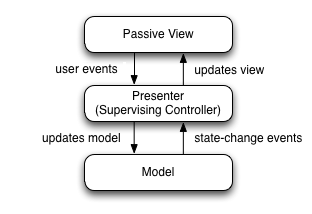
\includegraphics[]{image/1.png}
		\caption{MVP原理图}
	\end{figure}
	\begin{figure}[!h]
		\centering
		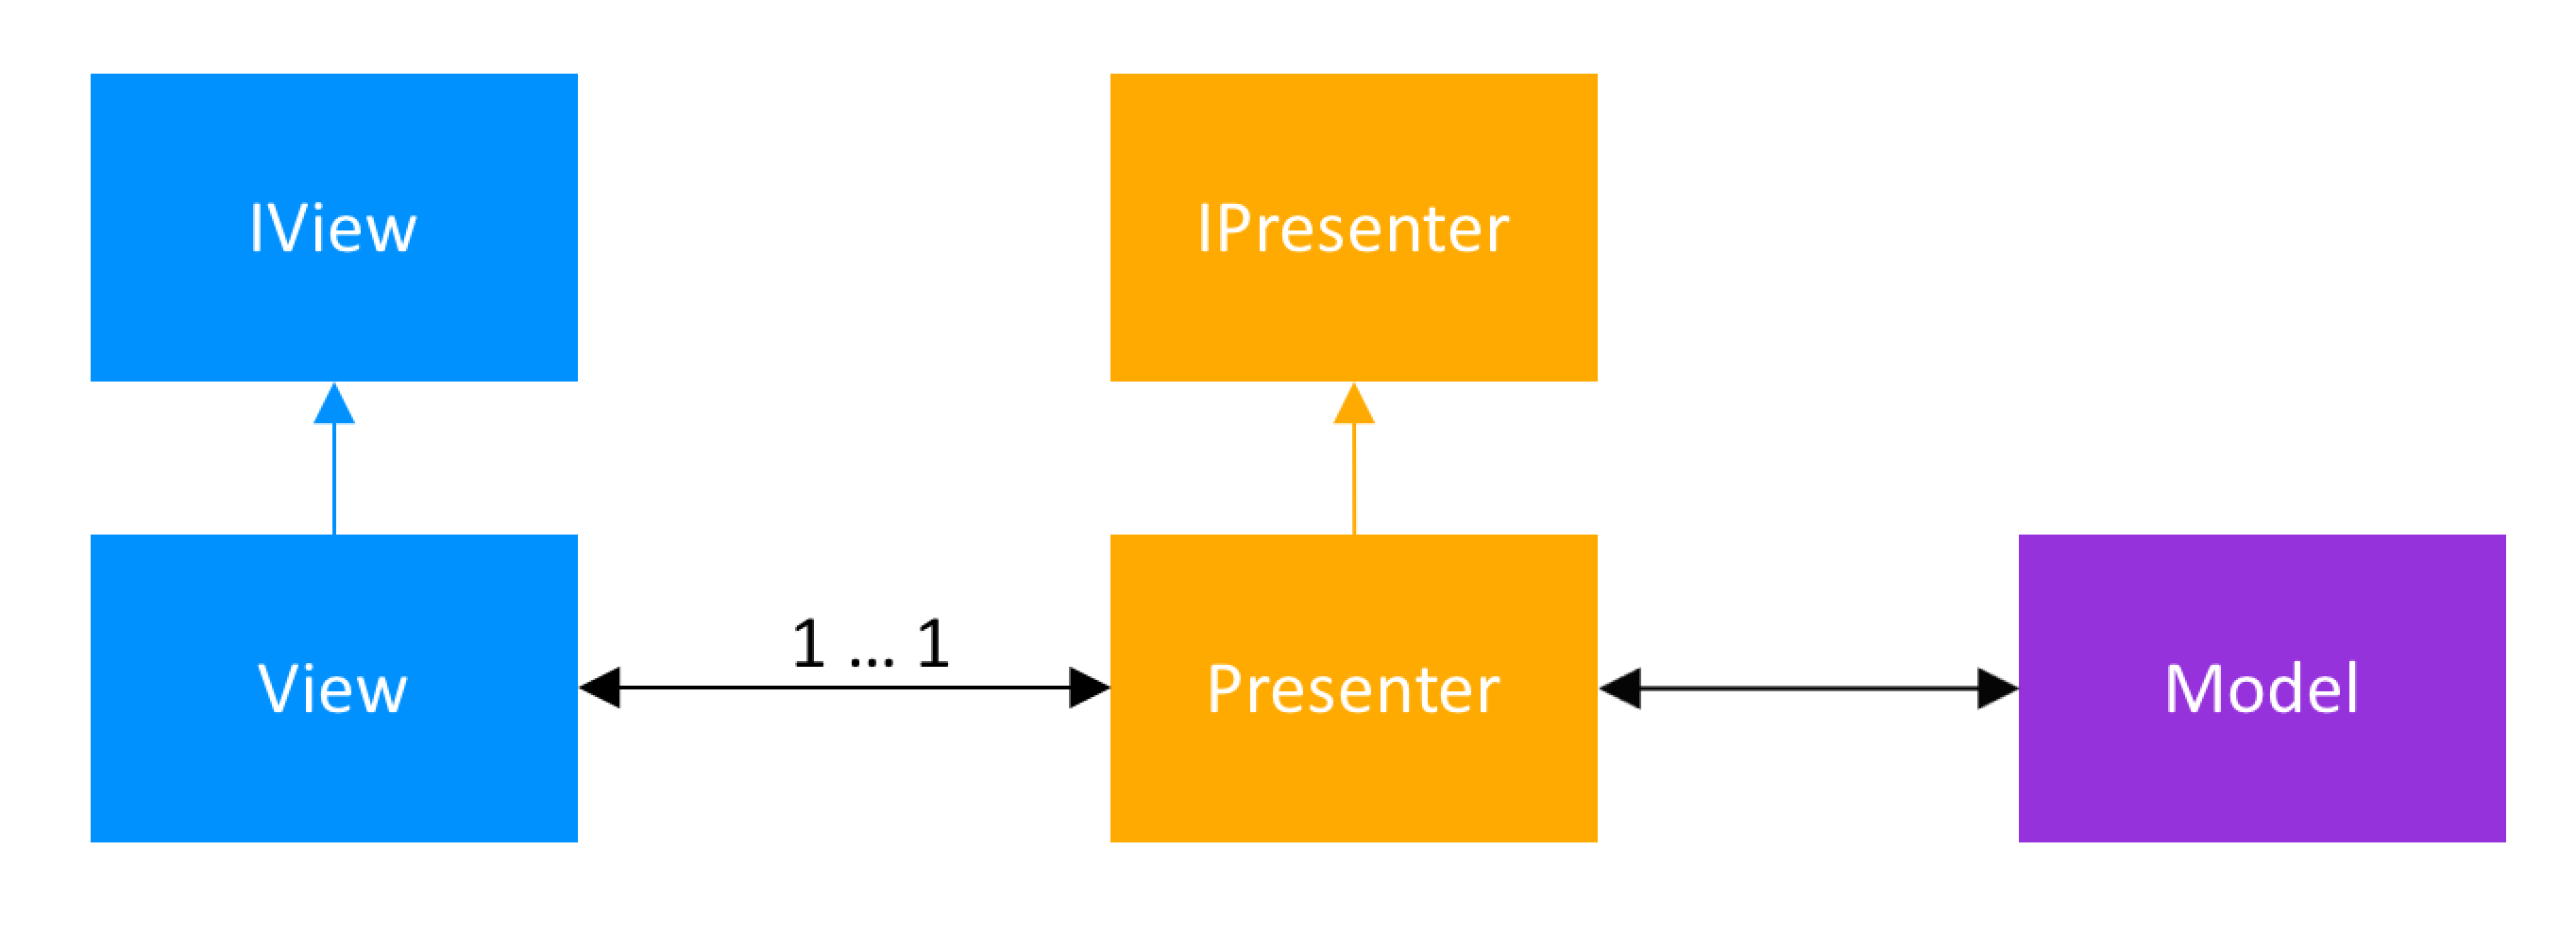
\includegraphics[width=0.8\textwidth]{image/2.png}
		\caption{Model-View-Presenter class structure}
	\end{figure}
	\subsection{优缺点}
	优点:
	\begin{enumerate}
		\item View与Model完全隔离,如果Model或View中的一方发生变化,只要交互接口不变,另一方就没必要对上述变化做出改变。这使得Model层的业务逻辑具有很好的灵活性和可重用性。
		\item Presenter与View的具体实现技术无关,采用诸如Windows表单、WPF、Web表单等用户界面构建技术中的任意一种来实现View层,都无需改变系统的其他部分。甚至为了使B/S,C/S部署架构能够被同时支持,应用程序可以用同一个Model层适配多种技术构建的View层。
		\item 可以进行View的模拟测试,在MVP模式中,View和Model之间没有直接依赖,开发者能够借助模拟对象注入测试两者中的任一方。
		\item 视图的变化总是比较频繁,将业务逻辑抽取出来,放在表示器中实现,使模块职责划分明显,层次清晰,一个表示器能复用于多个视图,而不需要更改表示器的逻辑,这增加了程序的复用性。
		\item 数据的处理由模型层完成,隐藏了数据,在数据显示时,表示器可以对数据进行访问控制,提高数据的安全性。
	\end{enumerate}
	\par 缺点:
	\par 增加了代码的复杂度,特别是针对小型Android应用的开发,会使程序冗余。
	\par 1. Presenter中除了应用逻辑以外,还有大量的View->Model,Model->View的手动同步逻辑,会导致Presenter臃肿,维护困难。
	\par 2. 视图的渲染过程也会放在Presenter中,造成视图与Presenter交互过于频繁,如果某特定视图的渲染很多,就会造成Presenter与该视图联系过于紧密,一旦该视图需要变更,那么Presenter也需要变更了,不能如预期的那样降低耦合度和增加复用性。
	\par 注:
	\begin{itemize}
		\item 如果要实现的UI比较复杂,而且相关的显示逻辑还跟Model有关系,就可以在View和Presenter之间放置一个Adapter。由这个Adapter来访问Model和View,避免两者之间的关联。而同时,因为Adapter实现了View的接口,从而可以保证与Presenter之间接口的不变。这样就可以保证View和Presenter之间接口的简洁,又不失去UI的灵活性。
		\item 在MVP模式里,View只应该有简单的Set/Get的方法,用户输入和设置界面显示的内容,除此就不应该有更多的内容,绝不容许直接访问Model--这就是与MVC很大的不同之处。
	\end{itemize}
	为什么MVP模式利于单元测试?
	\par Presenter将逻辑和UI分开了,里面没有Android代码,都是纯纯的java代码。我们可以直接对Presenter写Junit测试。
	\section{Android中的MVP}
	
\end{document}
